\vspace{1cm}
\fancyhead[C]{\normalsize\textbf{$\qquad$ Teil I: Offene Aufgaben}}
\renewcommand{\labelenumi}{\theenumi.}
\section*{Aufgabe 1 (40 Punkte)}
\vspace{0.4cm}
Ein institutioneller Anleger beabsichtigt im großen Stil Aktien einer Firma zu kaufen.
Da der Handelspreis der Aktie jedoch von der Nachfrage abhängt, möchte der Investor zuerst verstehen, wie seine Nachfrage den Preis beeinflussen wird.
Die Nachfrage des Investors in Abhängigkeit vom Preis ist gegeben durch $ d = D(p) =4 - 2 e^{p-1}$.
Der Preis der Aktie in Abhängigkeit von der Nachfrage $ d $ des Investors ist gegeben durch $ P(d) = \frac{1}{4} + \frac{1}{2} d $.
\subsection*{\aufgabe{a1}{2}}
Verknüpfen Sie die beiden Funktionen $ P $ und $ D $ zur Funktion $ Q = P \circ D $,
\begin{align*}
	Q : R_+ \to \R_{++} , \ p \mapsto q= Q(p),
\end{align*}
welche die Beziehung zwischen dem neuen Preis $ q $ und dem alten Preis $ p $ beschreibt,
nachdem der Investor $ D(p) $ Stück Aktien gekauft hat.
Geben Sie die Abbildungsvorschrift $ Q $ an.
\\
\\
\textbf{Lösung:}
\begin{mdframed}
\underline{\textbf{Vorgehensweise:}}
\renewcommand{\labelenumi}{\theenumi.}
\begin{enumerate}
\item Berechne die Verknüpfung der beiden Funktionen

\end{enumerate}
\end{mdframed}
\underline{1. Berechne die Verknüpfung der beiden Funktionen}\\
Um die Abbildungsvorschrift von $ Q $ zu bestimmen, müssen wir die Verknüpfung $ P \circ D $ berechnen.
Es gilt
\begin{align*}
	Q(p) = (P \circ D)(p)
	=
	P(D(p))
	=
	P(4 - 2e^{p-1})
	=
	\frac{1}{4} + \frac{1}{2}(4 - 2e^{p-1})
	=
	\frac{1}{4} + 2 -e^{p-1}
	=
	\frac{9}{4} - e^{p-1}
\end{align*}
für den Preis $ p \in \R_+ $.
Durch $ Q $ erhalten wir eine Funktion, welche den Preis der Aktie $ p = P(d) $ in Abhängigkeit von der Nachfrage $ d = D(p) $ beschreibt.
 


\newpage

\subsection*{\aufgabe{a2}{6}}
Zeigen Sie, dass es einen eindeutigen Fixpunkt $ p^\star \in \left[0,\frac{3}{2}\right] $ gibt, für welchen die Relation $ p^\star = Q(p^\star) $ gilt.
Gesucht ist also der Gleichgewichtspreis $ p^\star $, welcher unverändert bleibt, wenn der Investor $ D(p^\star ) $ Stück Aktien kauft.
\\ \\
\textbf{Lösung:}
\begin{mdframed}
\underline{\textbf{Vorgehensweise:}}
\renewcommand{\labelenumi}{\theenumi.}
\begin{enumerate}
\item Überlege dir, wie der Nullstellensatz von Bolzano anwendbar ist.
\item Zeige mit dem Nullstellensatz die Existenz eines Fixpunktes.
\item Zeige die Eindeutigkeit des Fixpunktes.
\end{enumerate}
\end{mdframed}

\underline{1. Überlege dir, wie der Nullstellensatz von Bolzano anwendbar ist}\\
Wir beginnen mit der Aussage des Nullstellensatzes von Bolzano.
Gegeben ist eine stetige Funktion $  f : [a,b] \to \R $ mit $ f(a) < 0 $ und $ f(b) > 0 $ (oder umgekehrt).
Dann existiert mindestens ein $ x \in [a,b] $, sodass $ f(x) = 0 $ ist.\\
Wir können also sagen, dass eine stetige Funktion mit wechselnden Vorzeichen mindestens eine Nullstelle dazwischen besitzt.\\
Unser Ziel ist nun nachzuweisen, dass genau ein $ p^\star \in \left[0,\frac{3}{2}\right] $ mit $ p^\star = Q(p^\star) $ existiert. Um den Nullstellensatz anzuwenden, behelfen wir uns mit der Funktion
\begin{align*} 
	f : \left[0,\frac{3}{2}\right] \to \R, \ p \mapsto f(p) = Q(p) - p
\end{align*}
und erhalten die Tatsache, dass
\begin{align*}
	 p = Q(p)  \ \Leftrightarrow \ 0 = Q(p) - p = f(p)
\end{align*}
gilt. Die Nullstellen von $ f $ entsprechen also den Fixpunkten von $ Q $ auf $ \left[0,\frac{3}{2}\right] $ und $ f $ ist stetig. Falls nun die Funktionswerte an den Intervallgrenzen unterschiedliche Vorzeichen besitzen, können wir den Nullstellensatz von Bolzano anwenden.\\
\\
\underline{2. Zeige mit dem Nullstellensatz die Existenz eines Fixpunktes}\\
Die Stetigkeit von $ f $ haben wir bereits abgeklärt. Für die Werte von $ f $ an den Grenzen des Intervalls gilt:
\begin{align*}
	f(0) &= Q(0) - 0 = \underbrace{\underbrace{\frac{9}{4}}_{> 2}- \underbrace{e^{-1}}_{< 1}}_{>0 } \approx 1.88 > 0\\
	f\left(\frac{3}{2}\right)
	&= 
	Q\left(\frac{3}{2}\right) - \frac{3}{2}
	=
	\frac{9}{4} - e^{\frac{3}{2} - 1} - \frac{6}{4}
	=
	\underbrace{\underbrace{\frac{3}{4}}_{< 1} - \underbrace{e^{\frac{1}{2}}}_{> 1}}_{< 0} \approx -0.90 <  0.
\end{align*}
Nach dem Nullstellensatz von Bolzano existiert mindestens ein $ p \in \left[0,\frac{3}{2}\right]  $ mit $ f(p) = 0$.\\
\\
\newpage
\underline{3. Zeige die Eindeutigkeit des Fixpunktes}\\
Bisher wurde abgeklärt das wir Fixpunkte von $ Q $ in $ \left[0,\frac{3}{2}\right] $ finden. Nun müssen wir nachweisen, dass nur ein solcher gefunden werden kann.
Falls $ f $ streng monoton ist, wissen wir das jeder Wert nur einmal von $ f $ angenommen werden kann.
Damit erhalten wir einen eindeutigen Fixpunkt. Es gilt
\begin{align*}
	f^\prime(p) = -e^{p-1} - 1 < 0
\end{align*}
für einen beliebigen Preis $ p $. Insbesondere ist $ f $ auf $ \left[0,\frac{3}{2}\right] $ streng monoton.\\
Alternativ ist $ f $ die Summe zweier streng monoton fallender Funktionen.\\
\\
Insgesamt haben wir gezeigt, dass wir einen eindeutigen Fixpunkt finden.
Damit existiert genau ein $ p^\star  \in \left[0,\frac{3}{2}\right]  $, sodass $ p^\star = Q(p^\star ) $ gilt.

\newpage
\subsection*{\aufgabe{a3}{6}}
Ein institutioneller Anleger beabsichtigt im großen Stil Aktien einer Firma zu kaufen.
Da der Handelspreis der Aktie jedoch von der Nachfrage abhängt, möchte der Investor zuerst verstehen, wie seine Nachfrage den Preis beeinflussen wird.
Die Nachfrage des Investors in Abhängigkeit vom Preis ist gegeben durch $ d = D(p) =4 - 2 e^{p-1}$.
Der Preis der Aktie in Abhängigkeit von der Nachfrage $ d $ des Investors ist gegeben durch $ P(d) = \frac{1}{4} + \frac{1}{2} d $.\\
Für die Funktion $ Q = P \circ D $ gibt es einen eindeutigen Punkt $ p^\star \in \left[0,\frac{3}{2}\right]  $ mit $ p^\star = Q(p^\star) $.\\
Verwenden Sie eine Taylor-Approximation zweiter Ordnung im Punkt $ p_0 = 1 $, um eine Näherung für $ p^\star  $ zu finden.
\\ \\
\textbf{Lösung:}
\begin{mdframed}
\underline{\textbf{Vorgehensweise:}}
\begin{enumerate}
\item Gebe zwei verschiedene Lösungswege an.
\item Lösungsweg nach Variante 1.
\item Lösungsweg nach Variante 2.
\item Bestimme die Annäherung an den Fixpunkt.
\end{enumerate}
\end{mdframed}

\underline{1. Gebe zwei verschiedene Lösungswege an}\\
Wir haben in den vorherigen Aufgaben bereits festgestellt, dass
\begin{align*}
	Q(p) = p \ \Leftrightarrow f(p) = 0
\end{align*}
mit $ f(p) = Q(p) - p  $ für $ p \in \left[0,\frac{3}{2}\right]   $ gilt.
Demnach lässt sich der Fixpunkt $ p^\star $ von $ Q $ über eine Taylor-Approximation von $ Q $  selbst oder über eine Taylor-Approximation von $ f $
annähern.
In der ersten Variante lösen wir ein Fixpunktproblem und in der zweiten Variante ein Nullstellenproblem für das jeweilig auftretende Taylorpolynom.\\
Wir werden jedoch sehen, dass beide Varianten äquivalent sind.\\
\\
\underline{2. Lösungsweg nach Variante 1}\\
Wir bestimmen nun das Taylorpolynom zweiter Ordnung $ P_{Q,2} $ im Punkt $ p_0 = 1 $.
Dieses ist schematisch durch
\begin{align*}
	P_{Q,2}(p)
	=
	Q(p_0) + Q^\prime(p_0)(p -p_0) + \frac{1}{2}Q^{\prime \prime}(p_0)(p-p_0)^2
	=
	Q(1)+ Q^\prime(1)(p -1) + \frac{1}{2}Q^{\prime \prime}(1)(p-1)^2
\end{align*}
gegeben. Es gilt $ Q(p) = \frac{9}{4} - e^{p-1} $.
Also folgt $ Q^{(k)}(p) = -e^{p-1} $ für $ k \geq 1 $ mithilfe der Kettenregel.
Das heißt, die Ableitungen ab der ersten Ordnung sind alle identisch.
Damit erhalten wir
\begin{align*}
	Q(1) &= \frac{9}{4} - e^{1-1} = \frac{9}{4} - 1 = \frac{5}{4}\\
	Q^\prime(1) &= Q^{\prime \prime}(1) =-  e^{1-1 } = e^0 =  - 1,
\end{align*}
woraus sich
\begin{align*}
	P_{Q,2}(p)
	&=
	\frac{5}{4} - (p - 1) - \frac{1}{2} (p - 1)^2 
	=
	\frac{5}{4} - p + 1 -\frac{1}{2}(p^2 - 2p +  1)
	=
	\frac{5}{4} - p + 1 - \frac{1}{2} p^2 + p - \frac{1}{2}\\
	&=
	- \frac{1}{2} p^2 + \frac{5}{4} + \frac{4}{4} - \frac{2}{4}
	=
	- \frac{1}{2} p^2 + \frac{7}{4} 
\end{align*}
ergibt. Damit entspricht das Fixpunktproblem einer quadratischen Gleichung:
\begin{align*}
	p = P_{Q,2}(p) = - \frac{1}{2} p^2 + \frac{7}{4} 
	\ \Leftrightarrow \
	- \frac{1}{2} p^2 - p  + \frac{7}{4} = 0
	\ \Leftrightarrow \
	\frac{1}{2} p^2 + p  - \frac{7}{4} = 0
	\ \Leftrightarrow \
	 p^2 + 2p  - \frac{7}{2} = 0.
\end{align*}
Wir werden nun hier die Notbremse ziehen und die zweite Variante auf die selbe quadratische Gleichung führen. Falls hieran kein Interesse besteht, kann gerne zu dem vierten Schritt gesprungen werden.\\
\\
\underline{3. Lösungsweg nach Variante 2}\\
Wir betrachten nun $ f(p) = Q(p) - p$ und erhalten:
\begin{align*}
	f(1) &= Q(1) - 1 = \frac{5}{4} -1 = \frac{1}{4}\\
	f^\prime(p) &= Q^\prime(p) - 1 \ \Rightarrow \
	f^\prime(1) = Q^\prime(1) - 1  = - 1 - 1 = -2\\
	f^{\prime \prime }(p) &= Q^{\prime \prime}(p) \ \Rightarrow \
		f^{\prime \prime }(1) = Q^{\prime \prime}(1) = -1.
\end{align*}
Damit ergibt die Taylor-Approximation von $ f $ in $ p_0 = 1 $:
\begin{align*}
	P_{f,2}(p)
	&=
	f(p_0) + f^\prime(p_0)(p -p_0) + \frac{1}{2}f^{\prime \prime}(p_0)(p-p_0)^2
	=
	\frac{1}{4} - 2 (p -1) - \frac{1}{2} p^2 + p - \frac{1}{2}\\
	&=
	\frac{1}{4} - 2p  + 2 - \frac{1}{2} p^2 + p - \frac{1}{2}\\
	&=
	- \frac{1}{2} p^2 - p + \frac{7}{4}.
\end{align*}
Unser Ziel ist nun, dass Nullstellenproblem
\begin{align*}
	0 = P_{f,2}(p) 
	\ \Leftrightarrow \
	- \frac{1}{2} p^2 - p + \frac{7}{4} = 0
	\ \Leftrightarrow \
	 p^2 +2 p - \frac{7}{2} = 0
\end{align*}
zu lösen. Dieses Problem ist äquivalent zu dem in Variante 1 auftretenden Fixpunktproblem.\\
\\
\underline{4. Bestimme die Annäherung an den Fixpunkt}\\
Wir wissen, dass wir durch das Lösen der Gleichung $  p^2 +2 p - \frac{7}{2} = 0 $ die Näherung an den Fixpunkt $ p^\star \in \left[0,\frac{3}{2}\right] $ erhalten.
Die Lösungen der Gleichung sind durch
\begin{align*}
	p^2 +2 p - \frac{7}{2} = 0
	\ \Leftrightarrow \
	p_{\nicefrac{1}{2}} 
	=  -1 \pm \sqrt{1 - \left(\frac{7}{2}\right)}
	=
	\ -1 \pm \sqrt{\frac{9}{2}}
\end{align*}
gegeben. Es gilt $ p_{-} = -1 - \sqrt{\frac{9}{2}}  < 0  $. Damit kommt nur $ p_+  $ infrage.
Für diese Lösung gilt:
\begin{align*}
	p_+ = -1 + \sqrt{\frac{9}{2}} \approx 1.12132 \approx p^\star. 
\end{align*}
Damit haben wir eine Näherung an den Fixpunkt $ p^\star  $ gefunden.


\newpage
\subsection*{\aufgabe{b}{6}}
Ein Computer hat eine Rechenleistung von $ a_n $ während der Periode $ n, \ n = 1,2,... $
Mithilfe maschinellen Lernens erhöht sich die Rechenleistung in jeder Periode um $ 2 \%  $, wobei sie zu Beginn $ a_1 = 10 $ beträgt.
Mit dem Computer benötigt die vollständige Berechnung einer bestimmten, anspruchsvollen Aufgabe $ 15 $ Perioden (d.h. die komplette Rechenleistung der ersten 15 Perioden wird für die Berechnung benötigt).\\
Anstelle die Berechnungen direkt zu starten, beschliesst das Rechenzentrum  zunächst die Rechenleistung des Computers aufzustocken.
Damit kann mit der Aufgabe zwar erst nach $ 3 $ Perioden begonnen werden, dafür aber hat der Computer nun eine neue anfängliche Rechenleistung von $ 15 $, welche sich pro Periode um $ 3 \% $ erhöht.\\
Wie viel Zeit (in Perioden) kann das Rechenzentrum durch das Aufstocken des Computers und den Aufschub der Berechnung einsparen?
\\ \\
\textbf{Lösung:}
\begin{mdframed}
\underline{\textbf{Vorgehensweise:}}
\begin{enumerate}
\item Bestimme die Rechenleistung der ersten 15 Perioden ohne die Verbesserung.
\item Bestimme die Anzahl der notwendigen Perioden nach der Verbesserung.
\end{enumerate}
\end{mdframed}

\underline{1. Bestimme die Rechenleistung der ersten 15 Perioden ohne die Verbesserung}\\
Um eine bestimmte, anspruchsvolle Rechenaufgabe zu lösen, benötigt der Computer 15 Perioden. Demnach ist die benötigte Rechenleistung durch
\begin{align*}
	s_{15}
	=
	\sum \limits_{n = 1}^\infty a_n 
	=
	a_1 +...+ a_{15}
\end{align*}
gegeben. Dies ist die $ 15. $ Partialsumme zur Folge $ \{a_n\}_{n \in \N} $.
Die Folge selbst ist rekursiv durch
\begin{align*}
	a_{n+1} = (1+ 2 \%) a_n = 1.02 \ a_n, \quad a_1 = 10
\end{align*}
definiert. Damit liegt eine geometrische Folge mit $ a_1  = 10$ und $ q =1.02 $ vor.
Also folgt
\begin{align*}
	s_{15}
	&=
	\sum \limits_{n = 1}^{15} a_n 
	=
	\sum \limits_{n = 1}^{15} a_1 q^{n-1} 
	=
	a_1 \sum \limits_{n = 1}^{15}  q^{n-1} 
	=
	a_1 \sum \limits_{n = 0}^{14}  q^{n}
	=
	a_1 \frac{1 - q^{14 + 1}}{1- q} 
	=
	10 \frac{1 - (1.02)^{15}}{1 - 1.02}\\
	&\approx 1729342
\end{align*}
mithilfe der geometrischen Summenformel.\\
Durch die Verbesserung erhalten wir die rekursive Vorschrift
\begin{align*}
	b_{n+1} = (1 + 3\%) b_n = 1.03 \ b_n
\end{align*}
mit der Ausgangsrechenleistung $ b_1 = 15 $. Dies ist eine geometrische Folge mit $ b_1 = 15 $ und $ \tilde{q} = 1.03 $
Die Rechenleistung nach $ n $ Perioden erhalten wir dann wieder mit der geometrischen Summenformel:
\begin{align*}
	\tilde{s}_n
	=
	\sum \limits_{k = 1}^n b_k
	=
	\sum \limits_{k = 1}^n b_1 \tilde{q}^{k-1}
	=
	b_1 \sum \limits_{k = 0}^{n-1}  \tilde{q}^{k}
	=
	b_1 \frac{1 - \tilde{q}^{n}}{1- \tilde{q}}
	=
	15 \frac{1 - (1.03)^n}{1- 1.03}.
\end{align*}
Wir wollen nach herausfinden wie viele Perioden nach der Verbesserung für die geforderte Rechenleistung notwendig sind.
Dies erhalten wir mit :
\begin{align*}
	\tilde{s}_n = s_{15}
	\ &\Leftrightarrow \
	15 \frac{1 - (1.03)^n}{1- 1.03} = s_{15}
	\ \Leftrightarrow \ 
	\frac{1 - (1.03)^n}{1- 1.03} = s_{15} \frac{1}{15}
	\ \Leftrightarrow \ 
	1 - (1.03)^n = s_{15} \frac{1- 1.03}{15}\\
	\ &\Leftrightarrow \ 
	 (1.03)^n = 1 -  s_{15} \frac{1- 1.03}{15}
	 \overset{(I)}{=}
	(1.02)^{15} 
	\ \Leftrightarrow \ 
	\ln(1.03^n) =  \ln (1.02^{15})\\
	\ &\Leftrightarrow \ 
	n \cdot \ln(1.03) =  \ln ((1.02)^{15})\\
	\ &\Leftrightarrow \ 
	n =  \frac{\ln (1.02^{15})}{\ln(1.03)}
	=15 \frac{\ln(1.02)}{\ln(1.03)}
	\approx 10.0491
\end{align*}
Damit braucht der verbesserte Computer ungefähr $ 10 $ Perioden um die Berechnung der Aufgabe abzuschließen. Da $ 3 $ Perioden zur Verbesserung benötigt werden erhalten wir eine Beschleunigung von $ 15 -10 -3  = 2 $ Perioden im Vergleich zu dem alten Computer.\\
\\
\textbf{\textit{Nebenrechnung (I):}}
\begin{align*}
	1 -  s_{15} \frac{1- 1.03}{15}
	&=
	1 - 10 \frac{1 - (1.02)^{15}}{1 - 1.02} \frac{1- 1.03}{15}
	=
	1 - \frac{2}{3}  \cdot \frac{1 - (1.02)^{15}}{-0.02} \cdot  (- 0.03)\\
	&=
	1 - \frac{2}{3} \cdot \frac{1 - (1.02)^{15}}{\frac{2}{100}} \cdot  \frac{3}{100}
	=
	1 - \frac{2}{3} \cdot (1 - (1.02)^{15} )\cdot  \frac{3}{100}  \frac{100}{2}\\
	&=
	1 - \frac{2}{3} \cdot (1 - (1.02)^{15} )\cdot  \frac{3}{2} 
	=
	(1.02)^{15} 
\end{align*}

\newpage
\subsection*{\aufgabe{c}{10}}
Eine Familie leiht sich CHF $ 1'000'000 $, um ein Haus zu kaufen.
Der Zins beträgt zu Beginn $ i = 1 \% $.
Die Familie beschliesst, CHF $ C_1 $ am Ende jeden Jahres für $ 10 $ Jahre zurückzuzahlen, um so den Schuldenstand auf CHF $ 750'000 $ am Ende des $ 10. $ Jahres zu reduzieren.
Am Ende des $ 5 $-ten Jahres ergibt sich die Möglichkeit einer Sondertilgung.
Die Familie zahlt folglich am Ende des $ 5 $-ten Jahres einen Gesamtbetrag von CHF $ 150'000 $ (einschliesslich $ C_1 $) zurück und verhandelt die Konditionen mit der Bank neu.
Der Zinssatz fällt damit auf $ 0.5 \% $.
Die Familie beschliesst, die Schulden weiterhin mit CHF $ C_1 $ am Ende jeden Jahres zurückzuzahlen, bis diese auf CHF $ 500'000 $ reduziert sind.
Aus steuerlichen Gründen zahlen sie anschliessend CHF $ C_2 $ pro Jahr an die Bank,
um ihre Schulden konstant bei CHF $ 500'000 $ zu halten.
\begin{enumerate}
	\item[(c1)]
	Fügen Sie alle Ereignisse und Mittelflüsse dem Zeitstrahl hinzu.
	\item[(c2)] 
	Berechnen Sie $ C_1 $.
	\item[(c3)] Wie hoch ist der Schuldenstand, nachdem die Familie die Zahlung von CHF 150'000 am Ende des $ 5 $-ten Jahres veranlasst hat?
	\item[(c4)] 
	Wie lange dauert es nach Ende des $ 5 $-ten Jahres, bis der Schuldenstand CHF $ 500'000 $ erreicht hat?
	\item[(c5)]
	Berechnen Sie $ C_2 $.
\end{enumerate}
\begin{center}
	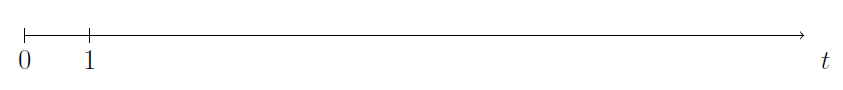
\includegraphics[scale=0.6]{pictures/zeitstrahl_1_c}
\end{center}
\ \\
\textbf{Lösung:}
\begin{mdframed}
	\underline{\textbf{Vorgehensweise:}}
	\begin{enumerate}
		\item[(c1)] Erstelle den Zeitstrahl.
		\item[(c2)] Berechne die jährliche Zahlung $ C_1 $.
		\item[(c3)] Bestimme den Schuldenstand nach der Sondertilgung.
		\item[(c4)] Bestimme die Anzahl an Jahren um einen Schuldenstand von $ 500'000 $ zu erreichen.
		\item[(c5)] Bestimme die Rate $ C_2 $ für einen konstanten Schuldenstand.
	\end{enumerate}
\end{mdframed}

\newpage
\underline{(c1) Erstelle den Zeitstrahl}\\
Der Zeitstrahl ist durch
\begin{center}
	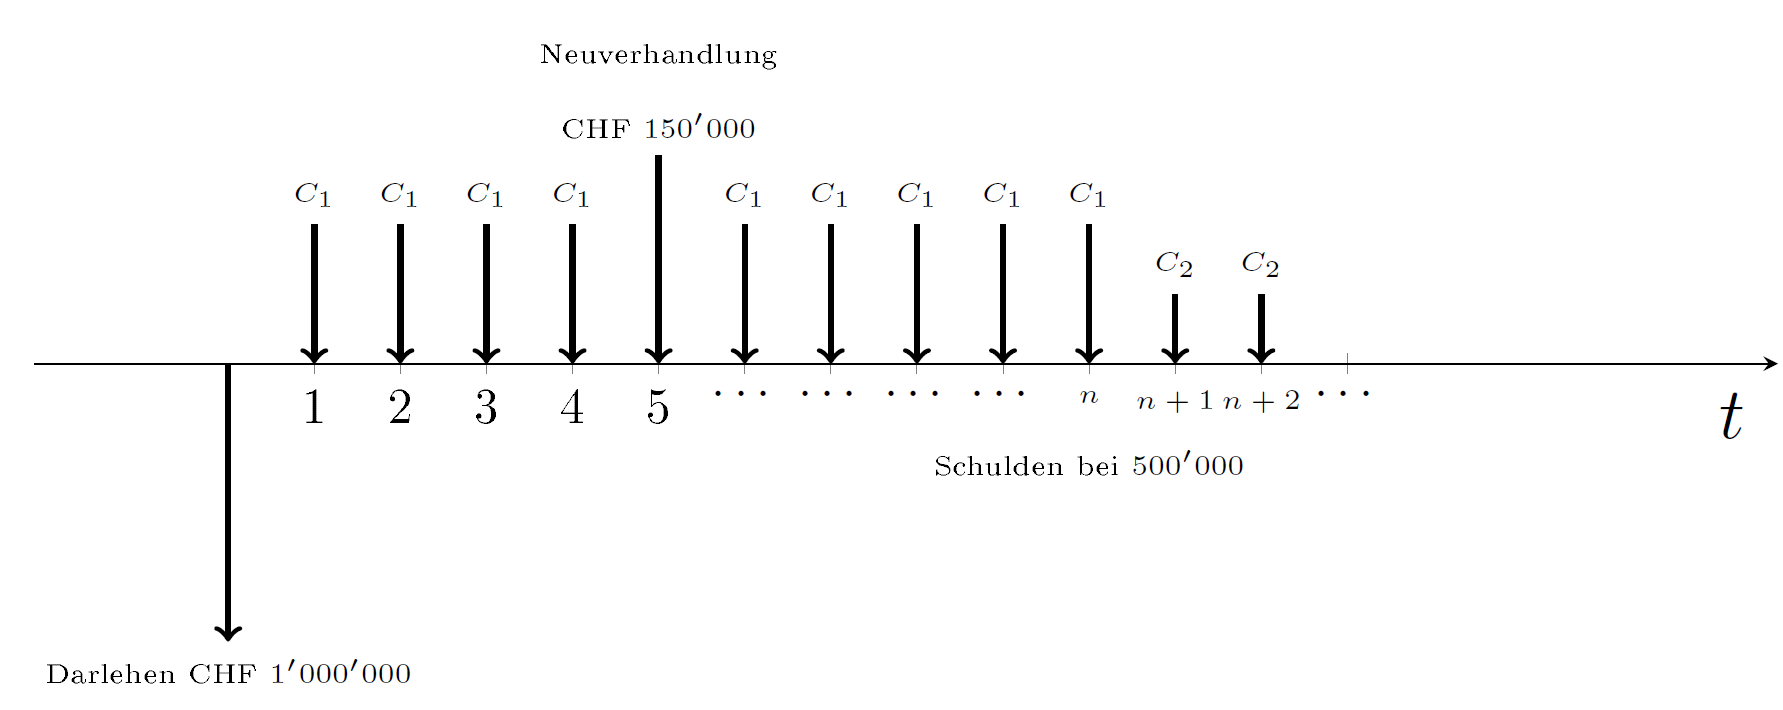
\includegraphics[scale=0.35]{pictures/zeitstrahl_1_c_filled}
\end{center}
gegeben. Damit ist die Teilaufgabe (c1) erledigt\\
\\
\underline{(c2) Berechne die jährliche Zahlung $ C_1 $}\\
Es war geplant, $ C_1 $ am Ende jeden Jahres über $ 10   $ Jahre zurückzuzahlen, sodass die Schulden von $ 1'000'000 $ CHF auf $ 750'000 $ reduziert werden.
Bei einem Zinssatz von $ 1\% $ ist ihm Jahre $ 10  $ der Betrag
\begin{align*}
	1'000'000(1+ 1 \%)^{10} - 750'000
	=
	1'000'000 \cdot 1.01^{10} -750'000
	\approx
	354'622.10
\end{align*}
zur Reduktion der Schulden notwendig. Dieser Wert muss nun einer nachschüssigen Rente mit jährlicher Zahlung $ C_1 $ nach $ 10 $ Jahren entsprechen.
Mit dem Endwert einer nachschüssigen Rente nach $ 10 $ Jahren erhalten wir:
\begin{align*}
	C_1 \frac{(1+ 1 \%)^{10}  - 1}{1 \%} = 354'622.10
	\
	\Leftrightarrow 
	\
	C_1 = \frac{1 \%}{(1+ 1 \%)^{10}  - 1} \cdot 354'622.10
	\approx 33'895.50 \ \mathrm{(CHF)}.
\end{align*}
Damit müssen jährlich ca. $ 33'895.50 $ CHF zurückgezahlt werden.\\
\\
\underline{(c3) Bestimme den Schuldenstand nach der Sondertilgung}\\
Den Schuldenstand nach $ 5  $ Jahren erhalten wir aus der über $ 5 $ Jahre verzinsten Kreditsumme abzüglich der über $ 5 $ Jahre getätigten Rückzahlung(Endwert nach $ 5 $ Zahlungen von $ C_1 $) und abzüglich 
der Sondertilgung $ 150'000 - C_1 $ CHF im fünften Jahr. Man beachte das einschliesslich in der Aufgabenstellung.
Damit ergibt sich für den Schuldenstand am Ende des fünften Jahres:
\begin{align*}
	&\underbrace{1'000'000(1+1 \%)^{5}}_{\textrm{Kreditsumme über } 5 \textrm{ Jahre verzinst}}
	-
	\underbrace{C_1 \frac{(1+ 1 \%)^{5}  - 1}{1 \%}}_{
	\textrm{Endwert nach $ 5 $ Jahren}
	}
	-
	\underbrace{(150'000 - C_1)}_{\textrm{Sondertilgung}}\\
	&\approx 1'051'010
	- 33'895.5 \frac{(1+ 1\%)^5 - 1}{1 \%} -150'000 + 33'895.5\\
	&\approx
	1'051'010
	-
	172'901.1
	-150'000 + 33'895.5\\
	&= 
	762'004.4 \ \textrm{(CHF)}.
\end{align*}
Am Ende des fünften Jahres hat die Familie eine Restschuld von $ 762'004.4 $ CHF.\\
\\
\newpage
\underline{(c4) Bestimme die Anzahl an Jahren um einen Schuldenstand von $ 500'000$ zu erreichen}\\
Nun ist die Frage nach wie vielen Jahren der Schuldenstand von $ 762'004.4 $ CHF auf 
$ 500'000 $ CHF sinkt.
Hierbei ist der neue Zinssatz durch $ i = 0.5 \% $ und die Jahresrate bleibt $ C_1 $.
Damit erhalten wir die Gleichung:
\begin{align*}
	\underbrace{500'000}_{\textrm{Zielschuldenstand}}
	&=
	\underbrace{762'004.4 (1+ 0.5 \%)^n}_{\textrm{Verzinsung über $ n $ Jahre}}
	-
	\underbrace{C_1 \frac{(1+ 0.5 \%)^{n}  - 1}{0.5 \%}}_{\textrm{Endwert nach $ n $ Jahren}}\\
	&=
	\left(762'004.4 - \frac{C_1}{0.5 \%} \right)(1+ 0.5 \%)^{n} + \frac{C_1}{0.5 \%}.
\end{align*}
Durch Auflösen der Gleichung nach $ n $ erhalten wir:
\begin{align*}
	&\left(762'004.4 - \frac{C_1}{0.5 \%} \right)(1+ 0.5 \%)^{n} = 500'000 -  \frac{C_1}{0.5 \%}\\
	\ \Leftrightarrow \
	&(1 + 0.5 \%)^n
	=
	\frac{500'000 -  \frac{C_1}{0.5 \%}}{762'004.4 - \frac{C_1}{0.5 \%}}\\
	\ \Leftrightarrow \
	&n  \ln(1 + 0.5 \%)
	=
	\ln\left(
	\frac{500'000 -  \frac{C_1}{0.5 \%}}{762'004.4 - \frac{C_1}{0.5 \%}}
	\right)
	= 
	\ln\left(500'000 -  \frac{C_1}{0.5 \%} \right)
	- 
	\ln\left(762'004.4 - \frac{C_1}{0.5 \%} \right)\\
	\ \Leftrightarrow \
	&n = 
	\frac{\ln\left(500'000 -  \frac{C_1}{0.5 \%} \right)
		- 
		\ln\left(762'004.4 - \frac{C_1}{0.5 \%} \right)}{\ln(1 + 0.5 \%)} \approx 8.54.
\end{align*}
Damit erreicht die Familie den Schuldenstand $ 9  $ Jahre nach der Sondertilgung bzw. dem Abschluss der neuen Konditionen.
Genau genommen ist die verbleibende Schuld nach $ 9 $ Jahren geringer als $ 500'000 $ CHF, denn es gilt:
\begin{align*}
	762'004.4 (1+ 0.5 \%)^9 - C_1 \frac{(1+ 0.5 \%)^{9}  - 1}{0.5 \%}
	\approx 485'756.1 \ \textrm{(CHF)}.
\end{align*}
Damit erhalten wir eine Interpretationsmöglichkeit, weswegen $ n = 8.54 $ und $ n  = 9 $ beides korrekte Antworten sind. In der nächsten Teilaufgabe rechnen wir mit einem Schuldenstand von $ 500'000 $ weiter.\\
\\
\underline{(c5) Bestimme die Rate $ C_2 $ für einen konstanten Schuldenstand}\\
Die Schulden von $ 500'000 $ bleiben konstant, wenn $ C_2 $ den anfallenden Zinsen entspricht. Also ist $ C_2 $ durch 
\begin{align*}
	C_2=  0.5 \% \cdot 500'000 = 2'500 \ \textrm{(CHF) }
\end{align*}
gegeben.\\
\\
Damit können sie als reicher Sack die Linkspartei für läppische $ 2'500 $ CHF verärgern, indem sie $ 2'500 $ CHF an dem Fiskus vorbeischleusen und diese stattdessen ihren Buddys von der Bank geben.
\newpage 

\subsection*{\aufgabe{d}{10}}
Ein Anbieter für Tablets schätzt die Nachfrage $ q_d $ nach seinem neusten Produkt auf
\begin{align*}
	q_d(p)
	=
	\frac{15'840 - 30 \ p}{p + 50},
\end{align*}
wobei $ p > 20  $ der Verkaufspreis in US-Dollar pro Tablet ist.
Die Kosten für Produktion und Vertrieb eines Tablets betragen $ 20  $ US-Dollar.
\begin{enumerate}
	\item[(d1)]
	Bestimmen Sie die Gewinnfunktion des Anbieters unter der Annahme, dass der Preis $ p > 20 $ ist.
	\item[(d2)]
	Leiten Sie die Funktion her, welche die Elastizität des Gewinns in Abhängigkeit vom Verkaufspreis beschreibt.
	\item[(d3)]
	Approximieren Sie mit Hilfe der Elastizitätsfunktion die relative Änderung des Gewinns bei einer Erhöhung des anfänglichen Verkaufspreises von $ p_0 = 100 $ US-Dollar um $ 5 $ US-Dollar.
\end{enumerate}

\ \\
\textbf{Lösung:}
\begin{mdframed}
	\underline{\textbf{Vorgehensweise:}}
	\begin{enumerate}
		\item[(d1)] Gebe die Gewinnfunktion an.
		\item[(d2)] Verwende einen Zusammenhang zwischen Kettenregel und der Logarithmusfunktion.
		\item[(d3)] Approximiere die relative Änderung durch die Elastizität.
	\end{enumerate}
\end{mdframed}

\underline{(d1) Gebe die Gewinnfunktion an}\\
Wir bezeichnen die Gewinnfunktion mit  $ G $. Diese Funktion besteht aus der Differenz aus Ertrag und Kosten. Mit $ E $ und $ K $ bezeichnen wir die Ertrags bzw. Kostenfunktion.
Damit gilt
\begin{align*}
	E(p) = q_d(p) \cdot p \ \textrm{und} \ K(p) = q_d(p) \cdot 20
\end{align*}
für $ p >20 $. 
Die Gewinnfunktion für $ p > 20 $ ergibt sich dann durch das Bilden der Differenz:
\begin{align*}
	G(p)
	= 
	E(p) -  K(p)
	=
	q_d(p) \cdot p - q_d(p) \cdot 20
	=
	q_d(p) \cdot (p -20)
	=
	\frac{15'840 - 30 \ p}{p + 50} (p -20).
\end{align*}
\ \\
\underline{(d2) Verwende einen Zusammenhang zwischen Kettenregel und der Logarithmusfunktion.}\\
Die Elastizität des Gewinns in Abhängigkeit des Preises $ p $ ist durch
\begin{align*}
	\varepsilon_{G}(p) = p \frac{G^\prime(p)}{G(p)}
\end{align*}
gegeben. Nun liegen zwei Möglichkeiten vor. Die Erste ist das (fehleranfällige) bestimmen der Ableitung von $ G $. Deswegen werden dies als Alternative durchführen.
Für die Zweite betrachten wir die aus der Kettenregel folgende Tatsache:
\begin{align*}
	(\ln(f(x)))^\prime = \frac{1}{f(x)} \cdot f^\prime(x)  = \frac{f^\prime(x)}{f(x)}.
\end{align*}
Wenn wir also die Ableitung von $ \ln(G(p))) $ bestimmen können, erhalten wir die Elastizität des Gewinns in Abhängigkeit des Preises $ p $ unmittelbar.
Hierfür formen wir zunächst $ \ln(G(p))) $ mit Logarithmusregeln um:
\begin{align*}
	\ln(G(p)))
	&=
	\ln \left(\frac{15'840 - 30  p}{p + 50} (p -20)\right)
	=
	\ln \left((15'840 - 30  p)(p -20) \frac{1}{p + 50}\right)\\
	&=
	\ln(15'840 - 30  p) + \ln(p -20) - \ln(p + 50).
\end{align*}
Damit vereinfacht sich das Differenzieren und  mit $\frac{30}{15'840} = \frac{1}{528}$ erhalten wir:
\begin{align*}
	(\ln(G(p))))^\prime
	&=
	(\ln(15'840 - 30 p) + \ln(p -20) - \ln(p + 50))^\prime
	=
	\frac{-30}{15'840 - 30 p} + \frac{1}{p -20} - \frac{1}{p + 50}\\
	&=
	\frac{1}{p - 528} + \frac{1}{p -20} - \frac{1}{p + 50}.
\end{align*}
Insgesamt ist die Elastizität durch
\begin{align*}
	\varepsilon_{G}(p) = p \frac{G^\prime(p)}{G(p)}
	= p \cdot 	(\ln(G(p))))^\prime 
	=
	\frac{p}{p - 528} + \frac{p}{p -20} - \frac{p}{p + 50}
\end{align*}
gegeben.\\
\\
Alternativ erhalten wir mit der Produkt-und Quotientenregel:
\begin{align*}
	G^\prime(p)
	&=
	\frac{(-30(p-20) + (15'840 - 30 p))(p+50) -(15'840 -30 p)(p-20) }{(p+50 )^2}\\
	&=
	\frac{-30(p-20)(p+50) + (15'840 - 30 p)(p+50- p + 20)}{(p+50 )^2}\\
	&=
	\frac{-30(p-20)(p+50) + 70 (15'840 - 30 p)}{(p+50 )^2}.
\end{align*}
Für die Elastizität folgt
\begin{align*}
	\varepsilon_{G}(p) = p \frac{G^\prime(p)}{G(p)}
	&=
	p \cdot \frac{-30(p-20)(p+50) + 70 (15'840 - 30 p)}{(p+50 )^2} \cdot 
	\frac{p +50}{(15'840 - 30 p)(p-20)}\\
	&=
	\frac{p}{p - 578} + \frac{70p}{(p+50)(p-20)}
\end{align*}
durch geschicktes Kürzen. Das dies der vorher bestimmten Elastizität entspricht lassen wir euch als (Bruchrechen-)Übungsaufgabe.\\
\\
\underline{(d3) Approximiere die relative Änderung durch die Elastizität}\\
Die relative Änderung von $ 100 $ USD auf $ 105 $USD des Gewinns ist durch 
\begin{align*}
	\frac{G(105) -G(100)}{G(100)}
\end{align*}
gegeben. Für diese gilt der Zusammenhang
\begin{align*}
	\frac{G(105) -G(100)}{G(100)}
	\approx
	\varepsilon_{G}(100) \frac{105- 100}{100} = \varepsilon_{G}(100) \cdot 5 \%
\end{align*}
mit der Elastizität.
Wegen 
\begin{align*}
	\varepsilon_{G}(100) = \frac{100}{100 - 528} + \frac{100}{100 - 20} - \frac{100}{100 + 50}
	\approx 0.35
\end{align*}
ergibt sich die ungefähre relative Änderung:
\begin{align*}
	\frac{G(105) -G(100)}{G(100)} \approx 0.35 \cdot 5 \% = 1.75 \%.
\end{align*}




\newpage